\section{Experiments with simulated data}
\label{simulation-studies}
\subsection{Estimators and evaluation metrics}
\label{sim-estimators}
We compare four variance estimators in two imputation families.  For
chained parametric MICE, RW-MICE denotes our stacked Robins--Wang
estimator (Section~\ref{extension-1}) and RR-MICE the Rubin's-rules
variance applied to the same imputations.  For predictive mean matching,
RW-PMM denotes the Robins--Wang estimator for use with PMM
(Section~\ref{extension-2}) and RR-PMM the Rubin's-rules variance
applied to the PMM imputations.  Within each RW/RR pair the point
estimator \(\hat\beta\) is identical; only the variance estimator
differs.
The two simulation settings are chosen to stress-test the two extensions
developed in Sections~\ref{extension-1}
and~\ref{extension-2} in
qualitatively different ways.
The first setting, the missing-data benchmark of \citet{robins2000inference},
uses ordinary outcome missingness and a linear analysis estimating equation.
Because the data-generating mechanism is well understood, we know in advance
which direction RR should fail: anti-conservative when the analysis
exploits heteroskedastic structure that the imputation model does not reflect
(panel~(b) of Figure~\ref{fig:schematic}), and conservative when the
imputation model is richer than the analysis (panel~(c)).  This allows the RW-MICE
extension to be evaluated against a known calibration benchmark rather than against
empirical performance alone.  The benchmark also includes PMM variants, which
assess whether the smooth copied-donor correction introduces any artefact under
ordinary missingness.
The second setting, the EHR validation setting of \citet{giganti2020multiple},
is a more demanding test that combines both extensions simultaneously.  Two
variables are imputed by MICE, one continuous and one binary.  The continuous
variable is imputed by either a Gaussian parametric model or by PMM; the binary
variable is imputed by a logistic conditional model.  Critically, the imputed
continuous variable determines both the analysis covariate and the eligibility
criterion for the analysis subset.  This imputation structure is
the canonical case of conservative uncongeniality: the imputation model is
fitted on all subjects, but the analysis equation is evaluated in a subset
whose membership fluctuates with the imputed values, inflating the
between-imputation variance for Rubin's rules.
For each simulation scenario, \(\beta^\ast\) denotes the large-sample target
of the implemented imputation-and-analysis procedure; in finite
simulation summaries it is approximated by the Monte Carlo mean of the
multiply imputed analysis estimator.  The primary variance calibration
measure is coverage of \(\beta^\ast\): for each replicate,
the usual confidence interval \(\hat\beta\pm1.96\widehat{SE}\) is
checked for coverage of \(\beta^\ast\).  This isolates variance
calibration from finite-sample bias.  We also report coverage of the
data-generating coefficient \(\beta_0\), mean bias
\(\hat\beta-\beta_0\), the empirical standard deviation of the Monte
Carlo estimates, and the mean estimated standard error.
Thus, coverage of \(\beta^\ast\)
answers whether the standard error estimates the sampling variability of
the implemented estimator, whereas coverage of \(\beta_0\) also reflects
finite-sample bias and target mismatch.  All simulations use 2500 Monte
Carlo replications per cell.
\subsection{Missing-data benchmark}
\label{simulation-rw-setting}
The missing-data benchmark follows the original simulation structure
used by RW: a hypothetical example involving children at a daycare
center.  Each subject has a group indicator \(A\), an
age covariate \(X\), and a continuous outcome \(Z\).
We use \(A=0\) for infants and \(A=1\) for toddlers, with
\(P(A=1)=1/3\).  Infants have \(X\sim U(0.1,0.8)\) and toddlers have
\(X\sim U(0.8,2.0)\).  In the main variants,
\[
  Z=X+\varepsilon,\qquad
  \varepsilon\mid X,A\sim N\{0,X^{\eta_A}\}.
\]
The outcome is fully observed for infants.  Among toddlers, \(Z\) is
missing with probability 0.60 except in the outcome-dependent
observation variant, where \(V=1\) denotes that \(Z\) is observed.  The
completed-data analysis is the no-intercept least-squares estimating
equation for the coefficient of \(X\) in \(E(Z\mid X)=\beta X\).  In
one variant the analysis is restricted to toddlers; otherwise all
subjects are included.  We generated data with both \(n=150\), matching
the original RW simulations exactly, and \(n=1000\).
The six scenarios are:
\[
\begin{array}{ll}
\text{S1:}  & \eta_0=\eta_1=0,\ \text{analysis restricted to toddlers};\\
\text{S2a:} & \eta_0=\eta_1=1,\ \text{all-subject analysis};\\
\text{S2b:} & \eta_0=\eta_1=-1,\ \text{all-subject analysis};\\
\text{S2c:} & \eta_0=2,\ \eta_1=1,\ \text{all-subject analysis};\\
\text{S3a:} & \eta_0=\eta_1=0,\ P(V=1\mid Z,A=1)=\expit(2-0.5Z);\\
\text{S3b:} & Z=X+0.5X^2+\varepsilon,\ \eta_0=\eta_1=0.
\end{array}
\]
S1 is the subgroup analysis case.  S2a--S2c retain the linear mean
analysis but change the variance relationship between the imputation
and analysis estimating equations.  S3a changes the observation
mechanism among toddlers, and S3b changes the outcome mean while
retaining the linear analysis.  In S3a and S3b, coverage of
\(\beta_0\) can differ from coverage of \(\beta^\ast\) because the
finite-sample estimator is centered away from the data-generating
coefficient.
Tables~\ref{tab:rw-benchmark-n150} and
\ref{tab:rw-benchmark-n1000} summarize the missing-data benchmark by
scenario.
For parametric MICE, RW/RR pairs compare RW-MICE with
RR-MICE.  For PMM, RW/RR pairs compare RW-PMM with
RR-PMM, using donor pool size \(k=5\).  RW-MICE has
coverage of \(\beta^\ast\) close to nominal in both sample size
settings.  RW-PMM shows the same pattern at \(n=1000\), with
coverage of \(\beta^\ast\) between 0.945 and 0.965 across the six
scenarios.  The \(n=150\) PMM cells are more variable, as expected for
small samples with copied donor values, but still correct the most
anti-conservative RR-PMM cells in S1, S2a, S2c, and S3b.  RR can be far from nominal: anti-conservative in S2a and S2c, and
conservative in S2b.  These results reproduce the key RW message in a
chained-equation implementation: when imputation and analysis
estimating equations are uncongenial, variance calibration depends on
the estimating-equation structure rather than on RR alone.

\begin{table}[ht]
\centering
\scriptsize
\setlength{\tabcolsep}{3.5pt}
\begin{tabular}{llrrrrrrr}
\toprule
Scenario & \makecell{Imputation\\model} & \makecell{Mean\\estimate} & Bias &
\makecell{Empirical\\SD} &
\makecell{Mean estimated SE\\RW/RR} &
\makecell{Coverage \(\beta^\ast\)\\RW/RR} &
\makecell{Coverage \(\beta_0\)\\RW/RR} & \makecell{Median corr.\\(score comp.)}\\
\midrule
S1  & Parametric MICE & 0.999 & -0.001 & 0.109 & 0.095 / 0.101 & 0.936 / 0.948 & 0.936 / 0.948 &\\
\addlinespace[1pt]
    & PMM (\(k=5\)) & 0.981 & -0.019 & 0.174 & 0.234 / 0.124 & 0.925 / 0.832 & 0.920 / 0.832 &\\
\addlinespace[1pt]
S2a & Parametric MICE & 0.998 & -0.002 & 0.108 & 0.095 / 0.066 & 0.942 / 0.806 & 0.943 / 0.804 &\\
\addlinespace[1pt]
    & PMM (\(k=5\)) & 0.990 & -0.010 & 0.164 & 0.182 / 0.104 & 0.926 / 0.783 & 0.925 / 0.778 &\\
\addlinespace[1pt]
S2b & Parametric MICE & 0.999 & -0.001 & 0.089 & 0.079 / 0.137 & 0.947 / 0.998 & 0.947 / 0.998 &\\
\addlinespace[1pt]
    & PMM (\(k=5\)) & 0.968 & -0.032 & 0.124 & 0.308 / 0.153 & 0.970 / 0.985 & 0.972 / 0.987 &\\
\addlinespace[1pt]
S2c & Parametric MICE & 0.998 & -0.002 & 0.107 & 0.094 / 0.055 & 0.945 / 0.722 & 0.945 / 0.718 &\\
\addlinespace[1pt]
    & PMM (\(k=5\)) & 0.992 & -0.008 & 0.168 & 0.165 / 0.097 & 0.913 / 0.736 & 0.916 / 0.731 &\\
\addlinespace[1pt]
S3a & Parametric MICE & 0.938 & -0.062 & 0.070 & 0.061 / 0.063 & 0.943 / 0.955 & 0.735 / 0.755 &\\
\addlinespace[1pt]
    & PMM (\(k=5\)) & 0.939 & -0.061 & 0.098 & 0.106 / 0.095 & 0.945 / 0.941 & 0.909 / 0.890 &\\
\addlinespace[1pt]
S3b & Parametric MICE & 1.670 & 0.670  & 0.097 & 0.085 / 0.086 & 0.944 / 0.941 & 0.002 / 0.002 &\\
\addlinespace[1pt]
    & PMM (\(k=5\)) & 1.667 & 0.667 & 0.147 & 0.140 / 0.109 & 0.931 / 0.858 & 0.012 / 0.002 &\\
\bottomrule
\end{tabular}
\caption{Missing-data benchmark at \(n=150\) and \(m=20\), with 2500
Monte Carlo replications per scenario.  Bias is the Monte Carlo mean
estimate minus the data-generating coefficient.  RW/RR pairs
refer to RW-MICE/RR-MICE for parametric MICE rows and
RW-PMM/RR-PMM for PMM rows.}
\label{tab:rw-benchmark-n150}
\end{table}

\begin{table}[ht]
\centering
\scriptsize
\setlength{\tabcolsep}{3.5pt}
\begin{tabular}{llrrrrrrr}
\toprule
Scenario & \makecell{Imputation\\model} & \makecell{Mean\\estimate} & Bias &
\makecell{Empirical\\SD} &
\makecell{Mean estimated SE\\RW/RR} &
\makecell{Coverage \(\beta^\ast\)\\RW/RR} &
\makecell{Coverage \(\beta_0\)\\RW/RR} & \makecell{Median corr.\\(score comp.)}\\
\midrule
S1  & Parametric MICE & 1.000 & -0.000 & 0.059 & 0.059 / 0.060 & 0.950 / 0.952 & 0.950 / 0.953 &\\
\addlinespace[1pt]
    & PMM (\(k=5\)) & 0.996 & -0.004 & 0.063 & 0.065 / 0.047 & 0.948 / 0.859 & 0.949 / 0.860 &\\
\addlinespace[1pt]
S2a & Parametric MICE & 0.999 & -0.001 & 0.059 & 0.060 / 0.040 & 0.952 / 0.812 & 0.952 / 0.810 &\\
\addlinespace[1pt]
    & PMM (\(k=5\)) & 1.000 & 0.000 & 0.065 & 0.065 / 0.041 & 0.952 / 0.784 & 0.952 / 0.785 &\\
\addlinespace[1pt]
S2b & Parametric MICE & 0.999 & -0.001 & 0.045 & 0.046 / 0.082 & 0.950 / 1.000 & 0.951 / 1.000 &\\
\addlinespace[1pt]
    & PMM (\(k=5\)) & 0.996 & -0.004 & 0.046 & 0.053 / 0.055 & 0.965 / 0.982 & 0.965 / 0.982 &\\
\addlinespace[1pt]
S2c & Parametric MICE & 0.999 & -0.001 & 0.059 & 0.059 / 0.034 & 0.955 / 0.725 & 0.953 / 0.726 &\\
\addlinespace[1pt]
    & PMM (\(k=5\)) & 0.999 & -0.001 & 0.064 & 0.064 / 0.039 & 0.945 / 0.762 & 0.945 / 0.760 &\\
\addlinespace[1pt]
S3a & Parametric MICE & 0.939 & -0.061 & 0.038 & 0.038 / 0.038 & 0.949 / 0.954 & 0.626 / 0.645 &\\
\addlinespace[1pt]
    & PMM (\(k=5\)) & 0.939 & -0.061 & 0.038 & 0.039 / 0.037 & 0.954 / 0.941 & 0.658 / 0.618 &\\
\addlinespace[1pt]
S3b & Parametric MICE & 1.672 & 0.672  & 0.052 & 0.052 / 0.052 & 0.953 / 0.945 & 0.000 / 0.000 &\\
\addlinespace[1pt]
    & PMM (\(k=5\)) & 1.688 & 0.688 & 0.054 & 0.055 / 0.042 & 0.954 / 0.868 & 0.000 / 0.000 &\\
\bottomrule
\end{tabular}
\caption{Missing-data benchmark at \(n=1000\) and \(m=50\), with 2500
Monte Carlo replications per scenario.  Columns are defined as in
Table~\ref{tab:rw-benchmark-n150}.}
\label{tab:rw-benchmark-n1000}
\end{table}

These results confirm that the MICE stacking construction
of Section~\ref{extension-1}
correctly captures the three RW variance sources under chained conditional
imputation.  Second, the RW-PMM estimator inherits this
calibration at \(n=1000\) and makes substantial improvements over
RR-PMM even at \(n=150\), where small sample variance is larger.  Both
estimators correctly distinguish between coverage of \(\beta^\ast\) (a
pure variance diagnostic, near-nominal for the proposed methods) and
coverage of \(\beta_0\) (which also reflects the bias of the implemented
estimator, and is low when \(\beta^\ast \neq \beta_0\) as in S3a and S3b).
The benchmark setting, however, does not fully stress test the PMM
correction.  The analysis subset does not depend on the imputed variable:
whether \(Z\) is large or small does not change which subjects enter the
least-squares estimating equation.  The donor-source correlation
adjustment (Section~\ref{donor-source-analysis-scores}) therefore has
limited impact in this setting, because the analysis-score contributions
of recipients with a common donor are not strongly correlated through a
shared eligibility event.  The GS validation setting below provides the
harder test, where the copied donor value simultaneously appears in the
analysis as a covariate and determines the analysis subset.
\clearpage
\subsection{Measurement-error validation setting}
\label{simulation-gs-setting}
The second simulation setting follows the GS electronic health record
validation example \citep{giganti2020multiple}.  The goal is to
estimate the association between a
continuous exposure \(A\) and a binary outcome \(D\).  Only error-prone
versions \(A^\ast\) and \(D^\ast\) are available for every subject, while
the validated variables \(A\) and \(D\) are observed in a validation
subset; the validated values are imputed for the remaining subjects.
The analysis model is a logistic regression of \(D\) on \(A\), restricted
to the post-imputation analysis set \(\{A>2\}\); the eligibility rule
reflects the common situation in which the study question concerns only
subjects above a clinical threshold on the (error-prone, then imputed)
exposure.  We generated data with \(n=2000\) and \(n=4000\), the latter matching the original GS implementation; the full sample-size grid \(n\in\{2000,4000,6000,8000\}\) for parametric MICE is shown in
Figure~\ref{fig:gs-parametric-full-supp}.
This setting is more demanding than the RW benchmark in three concrete
ways. First, there are two MICE blocks, one continuous and one binary,
so the stacking must handle a mixed-model chained structure with
cross-block nuisance terms as in
Section~\ref{extension-1}. Second, the eligibility rule \(\{A>2\}\)
means that the imputed \(A\) value determines whether a subject's
analysis score is zero or nonzero: two recipients copying from the same
donor therefore have correlated eligibility decisions and correlated
analysis score values, making this the setting where the donor source
adjustment of Section~\ref{donor-source-analysis-scores} matters most.
Third, the imputation model is fitted on all subjects while the analysis
runs only in the post imputation subset \(\{A>2\}\), the canonical
case of conservative uncongeniality, which inflates the between-imputation
variance through random subset membership, reproducing the panel~(c)
pattern of Figure~\ref{fig:schematic}.
As in the previous section, we implement both parametric and PMM
imputation.  In the parametric MICE cells, \(A\) is imputed from a Gaussian
conditional working model with predictors \(X_1,X_2,A^\ast,D^\ast\),
and \(D\) from a logistic model with the same predictors plus the
completed \(A\). In the PMM cells, only the continuous \(A\) block is
replaced by the smooth copied donor law; the \(D\) block remains
logistic. This design isolates the PMM correction: the binary block
contributes through the standard RW-MICE framework, while the donor source
adjustment applies only to the \(A\) block that directly drives eligibility.
Tables~\ref{tab:gs-validation-n2000} and
\ref{tab:gs-validation-n4000} report results separately by sample size.
Each table uses the same layout and presents three imputation models:
parametric MICE, PMM with \(k=5\), and PMM with \(k=10\).  We vary the
number of imputations \(m\in\{5,25,50,100\}\) to assess sensitivity to
the number of imputations, and the donor pool size \(k\) because it
governs how widely the smooth law spreads probability over donors;
Results for the larger donor pools \(k=20\) and \(k=30\) are reported
in Appendix~\ref{appendix-simulation-figures}
(Table~\ref{tab:pmm-k-sensitivity-supp};
Figure~\ref{fig:gs-pmm-current-n2000-supp}) and are broadly similar to
those for \(k=5\) and \(k=10\); results across sample sizes for
\(k=5\) are shown in Figure~\ref{fig:gs-pmm-current-k5-supp}.

\begin{table}[!htbp]
\centering
\scriptsize
\setlength{\tabcolsep}{2.5pt}
\begin{tabular}{rlrrrrrrr}
\toprule
\(m\) & \makecell{Imputation\\model} &
\makecell{Mean\\estimate} & Bias &
\makecell{Empirical\\SD} &
\makecell{Mean estimated SE\\RW/RR} &
\makecell{Coverage \(\beta^\ast\)\\RW/RR} &
\makecell{Coverage \(\beta_0\)\\RW/RR} & \makecell{Median corr.\\(score comp.)}\\
\midrule
5   & Parametric MICE & 0.850 & -0.040 & 0.120 & 0.114 / 0.166 & 0.937 / 0.985 & 0.900 / 0.973 &\\
5   & PMM (\(k=5\))  & 0.851 & -0.041 & 0.134 & 0.177 / 0.168 & 0.979 / 0.976 & 0.968 / 0.966 &\\
5   & PMM (\(k=10\)) & 0.842 & -0.046 & 0.136 & 0.149 / 0.169 & 0.956 / 0.978 & 0.944 / 0.962 &\\
\addlinespace[2pt]
25  & Parametric MICE & 0.850 & -0.040 & 0.109 & 0.107 / 0.162 & 0.944 / 0.996 & 0.910 / 0.985 &\\
25  & PMM (\(k=5\))  & 0.854 & -0.037 & 0.125 & 0.136 / 0.165 & 0.963 / 0.991 & 0.947 / 0.978 &\\
25  & PMM (\(k=10\)) & 0.843 & -0.048 & 0.127 & 0.129 / 0.166 & 0.956 / 0.989 & 0.923 / 0.973 &\\
\addlinespace[2pt]
50  & Parametric MICE & 0.850 & -0.040 & 0.108 & 0.107 / 0.162 & 0.946 / 0.998 & 0.907 / 0.984 &\\
50  & PMM (\(k=5\))  & 0.855 & -0.038 & 0.124 & 0.130 / 0.164 & 0.957 / 0.992 & 0.934 / 0.977 &\\
50  & PMM (\(k=10\)) & 0.843 & -0.048 & 0.125 & 0.126 / 0.165 & 0.946 / 0.989 & 0.929 / 0.978 &\\
\addlinespace[2pt]
100 & Parametric MICE & 0.850 & -0.040 & 0.107 & 0.106 / 0.162 & 0.944 / 0.998 & 0.909 / 0.986 &\\
100 & PMM (\(k=5\))  & 0.849 & -0.040 & 0.123 & 0.127 / 0.164 & 0.954 / 0.992 & 0.940 / 0.979 &\\
100 & PMM (\(k=10\)) & 0.843 & -0.048 & 0.124 & 0.124 / 0.165 & 0.953 / 0.991 & 0.934 / 0.986 &\\
\bottomrule
\end{tabular}
\caption{Measurement-error validation setting at \(n=2000\), with 2500
Monte Carlo replications per completed cell.  RW/RR pairs refer
to RW-MICE/RR-MICE for parametric MICE rows and
RW-PMM/RR-PMM for PMM rows.}
\label{tab:gs-validation-n2000}
\end{table}

\begin{table}[!htbp]
\centering
\scriptsize
\setlength{\tabcolsep}{2.5pt}
\begin{tabular}{rlrrrrrrr}
\toprule
\(m\) & \makecell{Imputation\\model} &
\makecell{Mean\\estimate} & Bias &
\makecell{Empirical\\SD} &
\makecell{Mean estimated SE\\RW/RR} &
\makecell{Coverage \(\beta^\ast\)\\RW/RR} &
\makecell{Coverage \(\beta_0\)\\RW/RR} & \makecell{Median corr.\\(score comp.)}\\
\midrule
5   & Parametric MICE & 0.869 & -0.020 & 0.083 & 0.082 / 0.117 & 0.944 / 0.989 & 0.921 / 0.980 &\\
5   & PMM (\(k=5\))  &       &        &       &               &               &               &\\
5   & PMM (\(k=10\)) &       &        &       &               &               &               &\\
\addlinespace[2pt]
25  & Parametric MICE & 0.869 & -0.021 & 0.076 & 0.078 / 0.115 & 0.951 / 0.996 & 0.920 / 0.992 &\\
25  & PMM (\(k=5\))  &       &        &       &               &               &               &\\
25  & PMM (\(k=10\)) &       &        &       &               &               &               &\\
\addlinespace[2pt]
50  & Parametric MICE & 0.869 & -0.021 & 0.075 & 0.077 / 0.115 & 0.950 / 0.995 & 0.920 / 0.992 &\\
50  & PMM (\(k=5\))  &       &        &       &               &               &               &\\
50  & PMM (\(k=10\)) &       &        &       &               &               &               &\\
\addlinespace[2pt]
100 & Parametric MICE & 0.869 & -0.021 & 0.075 & 0.077 / 0.114 & 0.956 / 0.997 & 0.925 / 0.992 &\\
100 & PMM (\(k=5\))  &       &        &       &               &               &               &\\
100 & PMM (\(k=10\)) &       &        &       &               &               &               &\\
\bottomrule
\end{tabular}
\caption{Measurement-error validation setting at \(n=4000\), with 2500
Monte Carlo replications per completed cell.  Columns are defined as in
Table~\ref{tab:gs-validation-n2000}.}
\label{tab:gs-validation-n4000}
\end{table}

\FloatBarrier
Tables~\ref{tab:gs-validation-n2000} and
\ref{tab:gs-validation-n4000} show that RW-MICE tracks the empirical
standard deviation more closely than RR in the parametric
MICE rows across all values of \(m\), confirming that the MICE
extension handles the conservative uncongeniality of this setting.
RR consistently overstates the standard error by
approximately 30--50\%, reproducing the GS finding at these larger
sample sizes (Figure~\ref{fig:gs-parametric}).
For PMM, the empirical rule concentrates the smooth law's probability
on approximately \(k\) donors while assigning positive probability to
the remainder; larger \(k\) spreads probability over more distant
donors. For the completed \(n=2000\) PMM rows,
RW-PMM standard errors are close to the empirical standard
deviation for \(m\ge 25\), while RR is conservative for
the same PMM point estimator.
Across the reported \(n=2000\) PMM validation cells with
\(k\in\{5,10,20,30\}\), coverage of \(\beta^\ast\) for RW-PMM ranges
from 0.943 to 0.979, compared with 0.976 to 0.992 for RR-PMM.  Coverage
of \(\beta_0\) is more sensitive to \(k\) because larger donor pools
admit more distant donors (a wider \emph{donor width}, i.e.\ the spread
of predictive means among eligible donors), which shifts the PMM point
estimator away from \(\beta_0\); this reflects donor-width bias rather
than variance miscalibration.  Results for the larger donor pools
\(k=20\) and \(k=30\) are reported in
Appendix~\ref{appendix-simulation-figures} and are broadly similar to
those for \(k=5\) and \(k=10\).
\subsection{Summary}
Across both settings the proposed RW estimators achieve near-nominal
coverage of \(\beta^\ast\) in most cases, while RR fails in
predictable directions: anti-conservative when the analysis exploits
structure the imputation model does not reflect, and conservative when
the imputation model uses information beyond the analysis. These failures are not
small: they reach 14--23 coverage-point shortfalls in the
anti-conservative direction (RW benchmark, S2a, S2c, S3b) and
approximately 30--50\% SE inflation in the conservative direction (GS
validation setting). The RW-PMM estimator inherits the
calibration of RW-MICE in the benchmark setting and correctly handles
the eligibility-by-imputation correlation structure in the GS setting,
with coverage of \(\beta^\ast\) between 0.943 and 0.979 across the
completed PMM cells. The distinction between coverage of \(\beta^\ast\)
and coverage of \(\beta_0\), illustrated in
Figure~\ref{fig:schematic} and maintained throughout the simulation
tables, is important: when the implemented estimator is biased for
\(\beta_0\) (as in S3a, S3b, and the GS validation setting), coverage
of \(\beta^\ast\) is the correct measure of variance calibration, and
the proposed RW methods achieve it.

\begin{figure}[ht]
\centering
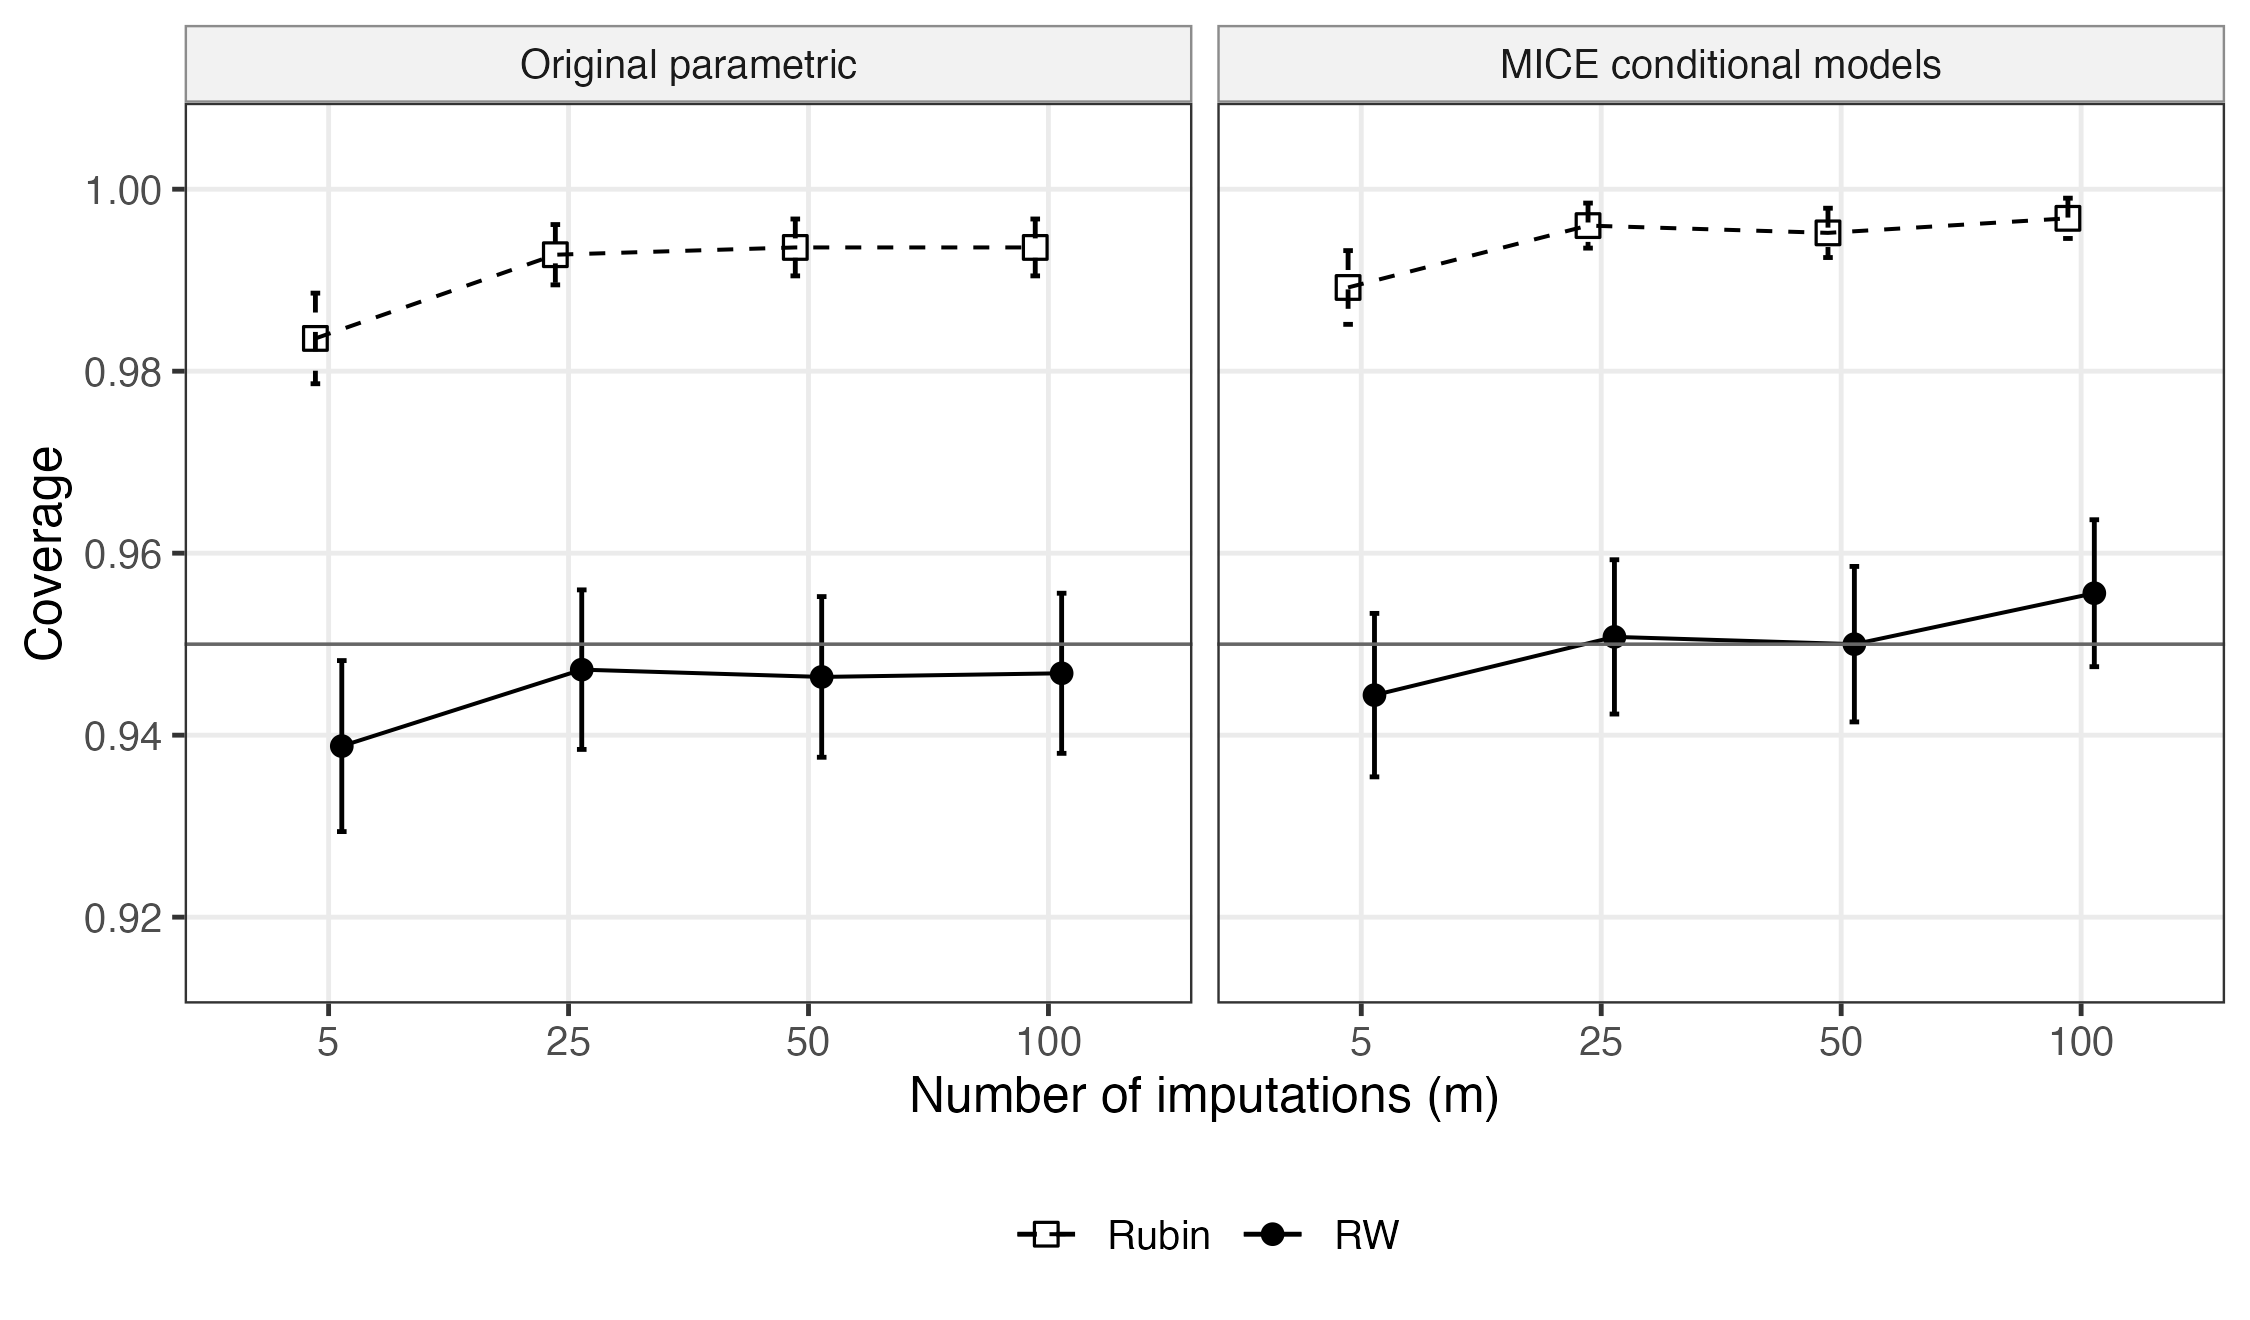
\includegraphics[width=\textwidth]{figures/gs_parametric_coverage_n4000.png}
\caption{Empirical-centered coverage in the Giganti--Shepherd
measurement-error setting with parametric imputation at \(n=4000\).
The left panel shows the original Giganti--Shepherd parametric
implementation, and the right panel shows the chained conditional MICE
implementation.}
\label{fig:gs-parametric}
\end{figure}

\clearpage
